\documentclass[10pt,a4paper]{article}
\input{AEDmacros}
\usepackage{etoolbox}
\usepackage{adjustbox}
\usepackage{inconsolata}
\usepackage{tcolorbox}
\usepackage{xcolor}
\usepackage{ragged2e}
\usepackage{changepage}
\usepackage{amssymb}
\usepackage[outputdir=out]{minted}
\DeclareRobustCommand{\ttfamily}{\fontencoding{T1}\fontfamily{lmtt}\selectfont}

\lstset{
  basicstyle=\ttfamily,
  numbers=none,
  frame=none,
  xleftmargin=10px,
  aboveskip=0pt
}
\newcommand{\vacio}{\emptyset}
\newcommand{\limn}{\lim_{n \to \infty}}
\newcommand{\ceil}[1]{%
  \left\lceil #1 \right\rceil%
}
\newcommand{\reales}{\mathbb{R}}
\newcommand{\limite}[2]{%
  \lim_{#1 \to #2}
}

\newenvironment{groupIzq}[1]{%
  \begin{list}{}{%
      \setlength{\leftmargin}{#1}%
      \setlength{\topsep}{0pt} % Elimina el espacio superior
      \setlength{\partopsep}{0pt} % Asegura que no haya espacio extra
    }
  \item[]
}{%
  \end{list}
}
\newcommand{\demoline}{\vspace{0.5em}}

\newcommand{\Indent}{\hspace*{0.75cm}}
\newcommand{\MiniIndent}{\hspace*{0.325cm}}
\newcommand{\Int}{\ensuremath{int}}

\newcommand{\Extends}[2]{%
  \noindent\ensuremath{\texttt{\textbf{#1}}\ \texttt{\textbf{extends}}\ #2}%
  \par
}
\newcommand{\Array}[1]{\ensuremath{Array \texttt{<}#1\texttt{>}}}
\newcommand{\Tupla}[1]{\ensuremath{Tupla \texttt{<}#1\texttt{>}}}
\newcommand{\Tuple}[1]{\ensuremath{Tuple \texttt{<}#1\texttt{>}}}
\newcommand{\Clase}[2]{\texttt{#1<#2>}}
\newcommand{\Type}[2]{%
  \noindent\ensuremath{\texttt{\textbf{#1}} = #2}%
  \par
}
\newcommand{\primitiva}[1]{\ensuremath{#1}}
\newcommand{\Arr}[1]{\ensuremath{Array \langle #1 \rangle}}
\newcommand{\conj}[1]{\ensuremath{conj \langle #1 \rangle}}
\newcommand{\union}{\cup}
\newcommand{\interseccion}{\cap}
\newcommand{\Struct}[1]{\ensuremath{\texttt{Struct} \langle \texttt{#1} \rangle}}
\newcommand{\StructField}[2]{\normalfont\ttfamily{#1}: \ensuremath{#2}}
\newcommand{\Title}[1]{%
  \raggedright
  \noindent{\textbf{#1}}%
  \justifying
  \vspace{1em}%
}

\newcommand{\TitlePar}[1]{%
  \raggedright
  \noindent{\textbf{#1}}%
  \justifying%
}

\newcommand{\Var}[2]{%
  \noindent\texttt{var \textbf{#1}}: #2 \par
}
\newenvironment{Vars}{%
  \begin{flushleft} % Alineación a la izquierda
}{%
  \end{flushleft}
  \vspace{1em} % Salto de línea final
}

\newenvironment{ModuloImplements}[2]{%
  \raggedright
  \texttt{Modulo #1\ implements\ #2\ \{}
  \justifying
  \begin{adjustwidth}{2em}{0em}
}{%
  \end{adjustwidth}
  \texttt{\}}%
}

\definecolor{lightgray}{gray}{1}
\definecolor{darkgray}{gray}{0.65}
\newcommand{\comentario}[1]{%
  \noindent{\normalfont\bfseries\ttfamily\small\textcolor{darkgray}{\% #1\ \ \%} \par}%
}

\newtcolorbox{ImplementationCodeBoxFixedWithParam}[1]{colback=lightgray!20, colframe=white, boxrule=0pt, left=5pt, right=5pt, top=5pt, bottom=5pt, width=#1}
\newtcolorbox{ImplementationCodeBoxFixed}{colback=lightgray!20, colframe=white, boxrule=0pt, left=5pt, right=5pt, top=5pt, bottom=5pt, width=0.8\linewidth}
\newtcolorbox{ImplementationCodeBox}{colback=lightgray!20, colframe=white, boxrule=0pt, left=5pt, right=5pt, top=5pt, bottom=5pt, width=\dimexpr\textwidth-2em\relax}
\definecolor{lightgray}{RGB}{220,220,220}
\newenvironment{ImplementationCode}[1]{%
  \VerbatimEnvironment
  \vspace{-0.2em}
  \begin{ImplementationCodeBoxFixedWithParam}{#1}
  \flushleft
  \begin{adjustbox}{minipage=\dimexpr\textwidth-2em\relax, margin=0pt}
  \begin{minted}[linenos, xleftmargin=-2.4em, numbersep=-2.5em]{java}%
}{
  \end{minted}
  \end{adjustbox}
  \vspace{-0.25em}
  \end{ImplementationCodeBoxFixedWithParam}
  \fussy
}

\usepackage{graphicx}
\usepackage{geometry}

\geometry{paperwidth=21cm, paperheight=80cm}

\begin{document}

\Title{Ejercicio 1}

\begin{figure}[h]
  \centering
  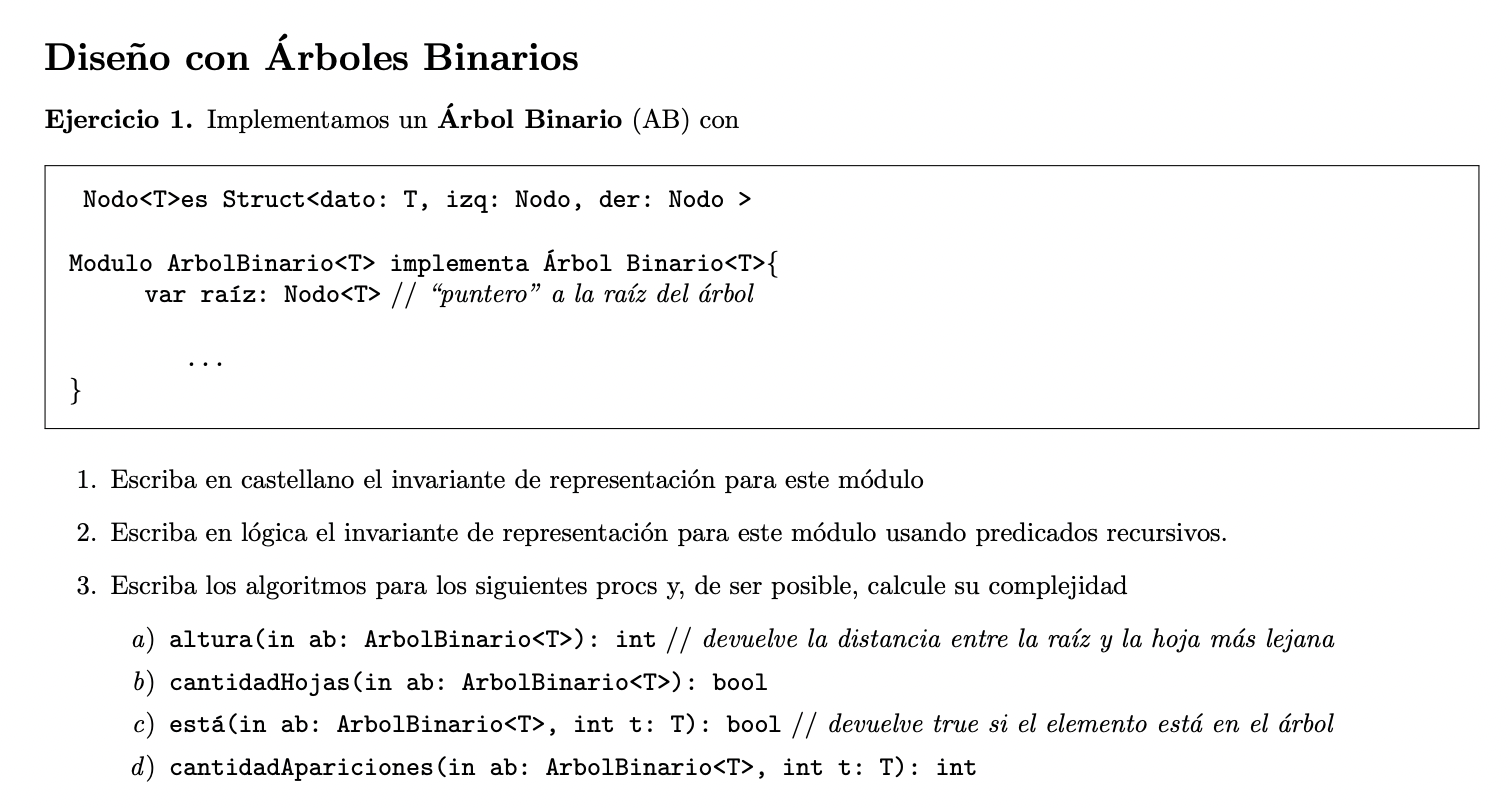
\includegraphics[width=\textwidth]{images/guia_7_ej_1.png}
  \caption{Enunciado Problema 1}
  \label{fig:ej_1}
\end{figure}

\begin{figure}[h]
  \centering
  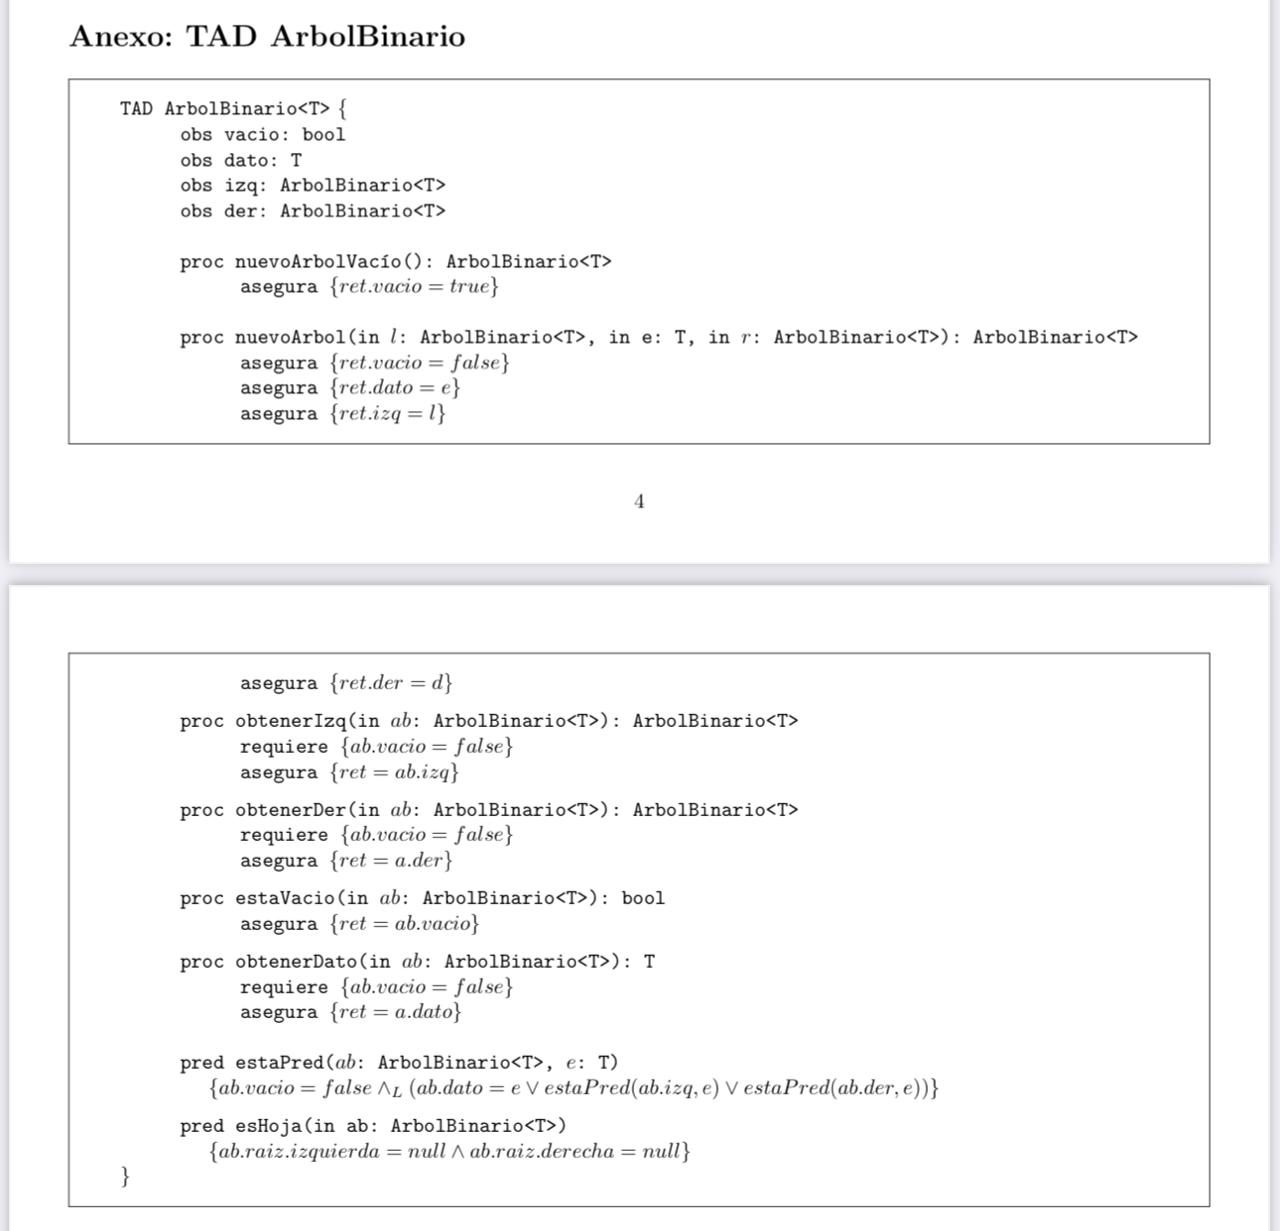
\includegraphics[width=\textwidth]{images/tad_arbol_binario.jpeg}
  \caption{TAD Arbol Binario<T>}
  \label{fig:tad_ab}
\end{figure}

\Extends{T}{\Clase{Comparable}{T}}
\Type{Nodo<T>}{\Struct{\StructField{valor}{T}, \StructField{izq}{\Clase{Nodo}{T}}, \StructField{der}{\Clase{Nodo}{T}}}}
\vspace{1em}
\begin{ModuloImplements}{ArbolBinarioImpl<T>}{ArbolBinario<T>}
  \begin{Vars}
    \Var{raiz}{\Clase{Nodo}{T}}
  \end{Vars}

  \pred{equivalentes}{raiz: \Clase{Nodo}{T}, ab': \Clase{ArbolBinario}{T}}{
    (raiz = null \land \neg def(ab')) \lor \\
    (
      \\\Indent raiz \neq null \land def(ab') \yLuego raiz.valor = ab'.dato \land 
      \\\Indent equivalentes(raiz.izq, ab'.izq) \land equivalentes(raiz.der, ab'.der)
    \\)
  }
  \pred{valoresDefinindos}{raiz: \Clase{Nodo}{T}}{
    raiz = Null \oLuego (raiz.valor \neq Null \land valoresDefinindos(raiz.izq) \land valoresDefinindos(raiz.der))
  }
  \aux{nodos}{raiz: \Clase{Nodo}{T}}{\conj{\Clase{Nodo}{T}}}{
    IfThenElse(
      \\\Indent raiz = null,
      \\\Indent \vacio,
      \\\Indent \{raiz\} \union nodos(raiz.izq) \union nodos(raiz.der),
    \\\hspace{0.65em})
  }
  \aux{cantidadPadres}{raiz: \Clase{Nodo}{T}, nodo: \Clase{Nodo}{T}}{\ent}{
    \\\Indent IfThenElse(
      \\\Indent\Indent raiz = null,
      \\\Indent\Indent 0,
      \\\Indent\Indent ifThenElse(
        \\\Indent\Indent\Indent raiz = nodo,
        \\\Indent\Indent\Indent 1,
        \\\Indent\Indent\Indent cantidadPadres(raiz.izq, nodo) + cantidadPadres(raiz.der, nodo),
      \\\Indent\Indent)
    \\\Indent)
  }
  \pred{tieneUnicoPadre}{raiz: \Clase{Nodo}{T}, nodo: \Clase{Nodo}{T}}{
    cantidadPadres(raiz, nodo) = 1
  }
  \pred{sinCiclos}{nodo: \Clase{Nodo}{T}, visitados: \conj{\Clase{Nodo}{T}}}{
    nodo = Null \oLuego (
      \\\Indent nodo \notin visitados \yLuego
      \\\Indent sinCiclos(nodo.izq, visitados \union \{nodo\}) \land
      \\\Indent sinCiclos(nodo.der, visitados \union \{nodo\})
    \\)
  }
  \comentario{Asumo que \ensuremath{ab'} no tiene ciclos}
  \pred{abs}{ab: \Clase{ArbolBinarioImpl}{T}, ab': \Clase{ArbolBinario}{T}}{
    (ab'.vacio == true \Leftrightarrow ab.raiz == Null) \land equivalentes(ab.raiz, ab')
  }
  \pred{invRep}{ab: \Clase{ArbolBinarioImpl}{T}}{
    sinCiclos(ab.raiz) \yLuego valoresDefinindos(ab.raiz) \land \\
    \paraTodo[unalinea]{nodo}{\Clase{Nodo}{T}}{nodo \in nodos(raiz) \implica tieneUnicoPadre(raiz, nodo)}
  }
  \vspace{1em}
  \comentario{Aux}
  \begin{proc}{auxMax}{\In a: int, \In b: int}{int}
    \begin{ImplementationCode}{320px}
      if a > b
        return a
      endif

      return b
    \end{ImplementationCode}
  \end{proc}
  \begin{proc}{auxEsHoja}{\In nodo: \Clase{Nodo}{T}}{int}
    \begin{ImplementationCode}{320px}
      return nodo.izq == null && nodo.der == null
    \end{ImplementationCode}
  \end{proc}
  \comentario{Fin Aux}
  \begin{proc}{alturaSubArbol}{\In ab: \Clase{ArbolBinarioImpl}{T}, \In nodo: \Clase{Nodo}{T}}{int}
    \begin{ImplementationCode}{320px}
      if nodo == null
        return 0
      endif

      return 1 + ab.auxMax(
        ab.alturaSubArbol(ab, nodo.izq),
        ab.alturaSubArbol(ab, nodo.der)
      )
    \end{ImplementationCode}
  \end{proc}
  \begin{proc}{altura}{\In ab: \Clase{ArbolBinarioImpl}{T}}{int}
    \begin{ImplementationCode}{320px}
      return ab.alturaSubArbol(ab, ab.raiz)
    \end{ImplementationCode}
  \end{proc}
  \vspace{2em}
  \begin{proc}{cantidadHojasSubArbol}{\In ab: \Clase{ArbolBinarioImpl}{T}, \In nodo: \Clase{Nodo}{T}}{int}
    \begin{ImplementationCode}{320px}
      if nodo == null then
        return 0
      endif

      if ab.auxEsHoja(nodo) then
        return 1
      endif

      return
        ab.cantidadHojasSubArbol(ab, nodo.izq) +
        ab.cantidadHojasSubArbol(ab, nodo.der)
    \end{ImplementationCode}
  \end{proc}
  \begin{proc}{cantidadHojas}{\In ab: \Clase{ArbolBinarioImpl}{T}}{int}
    \begin{ImplementationCode}{320px}
      return ab.cantidadHojasSubArbol(ab, ab.raiz)
    \end{ImplementationCode}
  \end{proc}
  \vspace{2em}
  \newpage
  \begin{proc}{estáEnSubArbol}{\In ab: \Clase{ArbolBinarioImpl}{T}, \In nodo: \Clase{Nodo}{T}, \In t: T}{bool}
    \begin{ImplementationCode}{320px}
      if nodo == null then
        return false
      endif

      return nodo.valor.compareTo(t) == 0
        || ab.estáEnSubArbol(ab, nodo.izq, t)
        || ab.estáEnSubArbol(ab, nodo.der, t)
    \end{ImplementationCode}
  \end{proc}
  \begin{proc}{está}{\In ab: \Clase{ArbolBinarioImpl}{T}, \In t: T}{bool}
    \begin{ImplementationCode}{320px}
      return ab.estáEnSubArbol(ab, ab.raiz, t)
    \end{ImplementationCode}
  \end{proc}
  \vspace{2em}
  \begin{proc}{cantidadAparicionesEnSubArbol}{\In ab: \Clase{ArbolBinarioImpl}{T}, \In nodo: \Clase{Nodo}{T}, \In t: T}{int}
    \begin{ImplementationCode}{320px}
      if nodo == null then
        return 0
      endif

      var cantidadAparicionesEnSubArboles: int
          cantidadAparicionesEnSubArboles:=
            ab.cantidadAparicionesEnSubArbol(ab, nodo.izq, t) +
            ab.cantidadAparicionesEnSubArbol(ab, nodo.der, t)

      if nodo.valor.compareTo(t) == 0 then
        return 1 + cantidadAparicionesEnSubArboles
      endif

      return cantidadAparicionesEnSubArboles
    \end{ImplementationCode}
  \end{proc}
  \begin{proc}{cantidadApariciones}{\In ab: \Clase{ArbolBinarioImpl}{T}, \In t: T}{int}
    \begin{ImplementationCode}{320px}
      return ab.cantidadAparicionesEnSubArbol(ab, ab.raiz, t)
    \end{ImplementationCode}
  \end{proc}
\end{ModuloImplements}

\newpage

\begin{figure}[h]
  \centering
  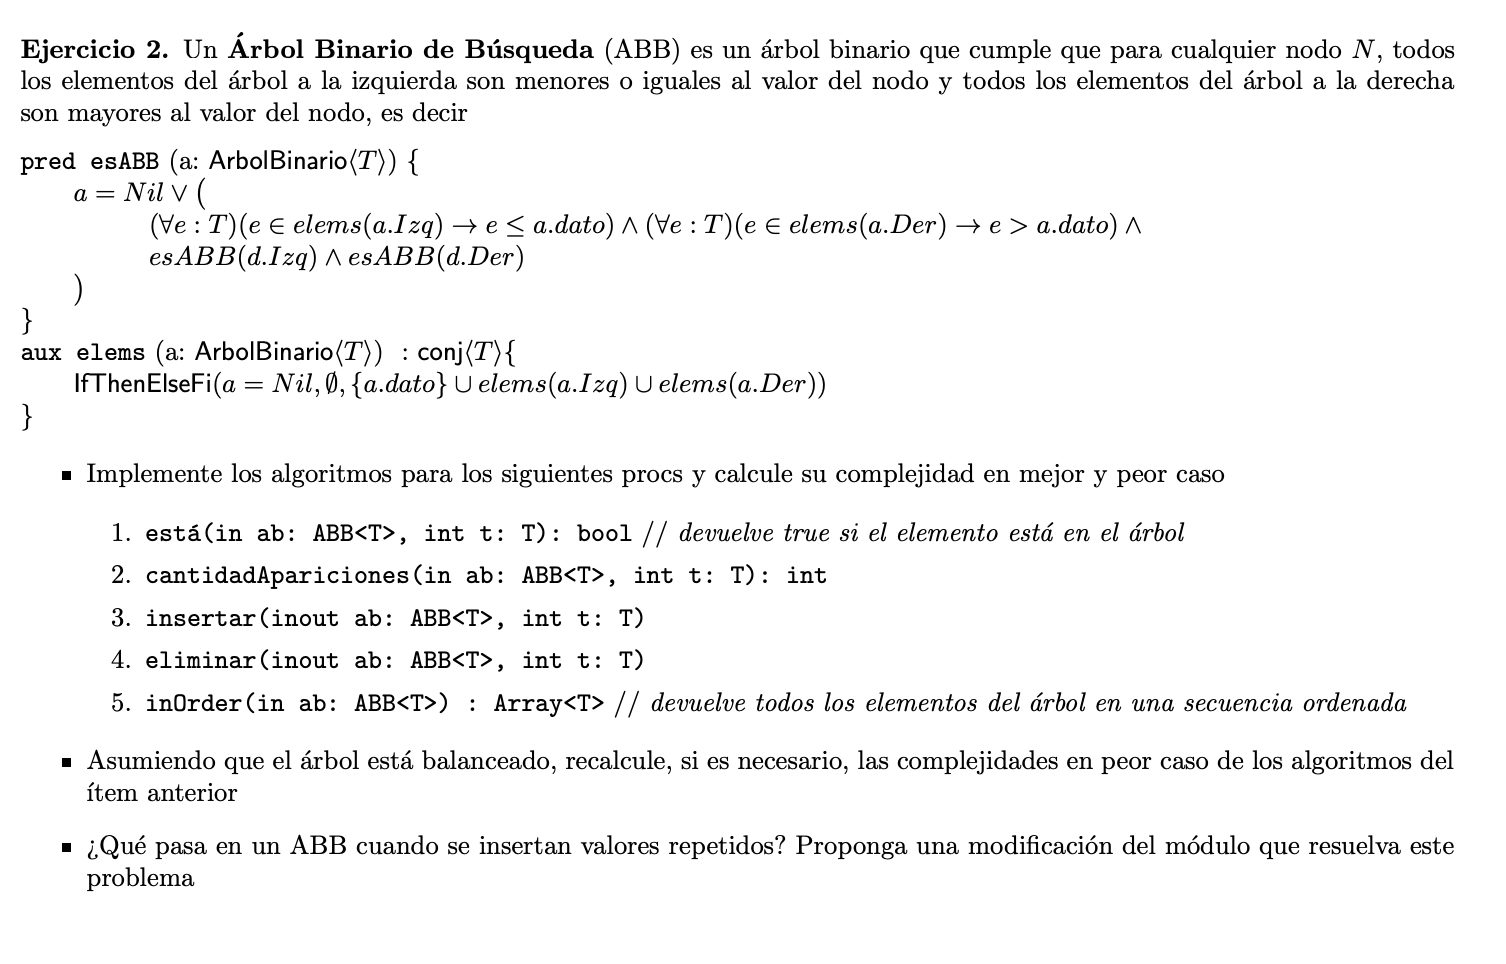
\includegraphics[width=\textwidth]{images/guia_7_ej_2.png}
  \caption{Ejercicio 2}
  \label{fig:ej_2}
\end{figure}

\Extends{T}{\Clase{Comparable}{T}}
\Type{Nodo<T>}{\Struct{\StructField{valor}{T}, \StructField{izq}{\Clase{Nodo}{T}}, \StructField{der}{\Clase{Nodo}{T}}}}
\vspace{1em}
\begin{ModuloImplements}{ABB<T>}{ArbolBinario<T>}
  \begin{Vars}
    \Var{raiz}{\Clase{Nodo}{T}}
  \end{Vars}
  \comentario{Aux}
  \begin{proc}{auxTieneDosHijos}{\In nodo: \Clase{Nodo}{T}}{int}
    \begin{ImplementationCode}{320px}
      return nodo.izq != null && nodo.der != null
    \end{ImplementationCode}
  \end{proc}
  \begin{proc}{auxMaximoSubArbol}{\In nodo: \Clase{Nodo}{T}}{T}
    \begin{ImplementationCode}{320px}
      if nodo.der != null then
        return auxMaximoSubArbol(nodo.der)
      endif

      return nodo.valor
    \end{ImplementationCode}
  \end{proc}
  \begin{proc}{auxColaAArray}{\In cola: \Clase{ColaSobreLista}{T}, \In tamañoCola: int}{\Array{T}}
    \begin{ImplementationCode}{320px}
      res:= new Array<T>(tamañoCola)
      
      var i: int
          i:= 0

      while (!cola.colaVacía()) do
        res[i]:= cola.desencolar()
        i:= i + 1
      endwhile

      return res
    \end{ImplementationCode}
  \end{proc}
  \comentario{Fin Aux}
  \begin{proc}{estáEnSubArbol}{\In abb: \Clase{ABB}{T}, \In nodo: \Clase{Nodo}{T}, \In t: T}{bool}
    \begin{ImplementationCode}{320px}
      if nodo == null then
        return false
      endif

      if nodo.valor.compareTo(t) < 0 then
        return abb.estáEnSubArbol(abb, nodo.izq, t)
      endif

      if nodo.valor.compareTo(t) > 0 then
        return abb.estáEnSubArbol(abb, nodo.der, t)
      endif

      return true
    \end{ImplementationCode}
  \end{proc}
  \begin{proc}{está}{\In abb: \Clase{ABB}{T}, \In t: T}{bool}
    \begin{ImplementationCode}{320px}
      return abb.estáEnSubArbol(abb, abb.raiz, t)
    \end{ImplementationCode}
  \end{proc}
  \vspace{2em}
  \begin{proc}{cantidadAparicionesEnSubArbol}{\In abb: \Clase{ABB}{T}, \In nodo: \Clase{Nodo}{T}, \In t: T}{int}
    \begin{ImplementationCode}{380px}
      if nodo == null then
        return 0
      endif

      if nodo.valor.compareTo(t) <= 0 then
        if nodo.valor.compareTo(t) == 0 then
          return 1 + abb.cantidadAparicionesEnSubArbol(abb, nodo.izq, t)
        endif

        return abb.cantidadAparicionesEnSubArbol(abb, nodo.izq, t)
      endif

      return abb.cantidadAparicionesEnSubArbol(abb, nodo.der, t)
    \end{ImplementationCode}
  \end{proc}
  \begin{proc}{cantidadApariciones}{\In abb: \Clase{ABB}{T}, \In t: T}{int}
    \begin{ImplementationCode}{360px}
      return abb.cantidadAparicionesEnSubArbol(abb, abb.raiz, t)
    \end{ImplementationCode}
  \end{proc}
  \vspace{2em}
  \begin{proc}{insertarEnSubArbol}{\Inout abb: \Clase{ABB}{T}, \In nodo: \Clase{Nodo}{T}, \In t: T}{\Clase{Nodo}{T}}
    \begin{ImplementationCode}{320px}
      if nodo == null then
        var nodo: Nodo<T>
            nodo:= new Nodo()
        
        nodo.valor:= t

        return nodo
      endif

      if nodo.valor.compareTo(t) >= 0 then
        nodo.izq:= abb.insertarEnSubArbol(abb, nodo.izq, t)
      else
        nodo.der:= abb.insertarEnSubArbol(abb, nodo.der, t)
      endif

      return nodo
    \end{ImplementationCode}
  \end{proc}
  \begin{proc}{insertar}{\Inout abb: \Clase{ABB}{T}, \In t: T}{}
    \begin{ImplementationCode}{320px}
      abb.raiz:= abb.insertarEnSubArbol(abb, abb.raiz, t)

      return
    \end{ImplementationCode}
  \end{proc}
  \vspace{2em}
  \begin{proc}{eliminarDelSubArbol}{\Inout abb: \Clase{ABB}{T}, \In nodo: \Clase{Nodo}{T}, \In t: T}{\Clase{Nodo}{T}}
    \begin{ImplementationCode}{420px}
      if nodo.valor.compareTo(t) > 0 then
        nodo.izq:= eliminarDelSubArbol(abb, nodo.izq, t)
      else if nodo.valor.compareTo(t) < 0 then
        nodo.der:= eliminarDelSubArbol(abb, nodo.der, t)
      else
        // Acá se encontró un potencial nodo a eliminar
        if abb.auxTieneDosHijos(nodo) then
          nodo.valor:= abb.auxMaximoSubArbol(nodo.izq)
          nodo.izq:= eliminarDelSubArbol(abb, nodo.izq, nodo.valor)
        else
          // Acá puedo tener 3 casos: a) Hijo izq; b) Hijo der; c) Hijos null
          return nodo.izq != null ? nodo.izq : nodo.der
        endif
      endif

      return nodo
    \end{ImplementationCode}
  \end{proc}
  \begin{proc}{eliminar}{\Inout abb: \Clase{ABB}{T}, \In t: T}{}
    \begin{ImplementationCode}{320px}
      abb.raiz:= eliminarDelSubArbol(abb, abb.raiz, t)

      return
    \end{ImplementationCode}
  \end{proc}
  \vspace{2em}
  \begin{proc}{inorderSubArbol}{\Inout cola: \Clase{ColaSobreLista}{T}, \In abb: \Clase{ABB}{T}, \In nodo: \Clase{Nodo}{T}}{int}
    \begin{ImplementationCode}{320px}
      if nodo == null then
        return 0
      endif

      var tamañoIzq: int
      var tamañoDer: int

      tamañoIzq:= inorderSubArbol(cola, abb, nodo.izq)
      cola.encolar(nodo.valor)
      tamañoDer:= inorderSubArbol(cola, abb, nodo.der)

      return 1 + tamañoIzq + tamañoDer
    \end{ImplementationCode}
  \end{proc}
  \newpage
  \begin{proc}{inorder}{\In abb: \Clase{ABB}{T}}{\Array{T}}
    \begin{ImplementationCode}{320px}
      var cola: ColaSobreLista<T>
          cola:= new colaVacía()

      var tamañoCola: int
          tamañoCola:= abb.inorderSubArbol(cola, abb, abb.raiz)

      return abb.auxColaAArray(cola, tamañoCola)
    \end{ImplementationCode}
  \end{proc}
\end{ModuloImplements}

\newpage

\begin{figure}[h]
  \centering
  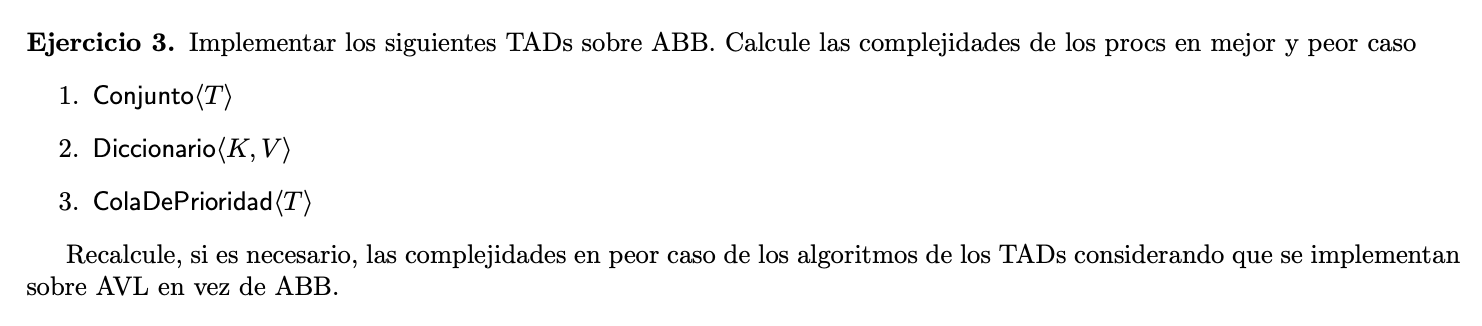
\includegraphics[width=\textwidth]{images/guia_7_ej_3.png}
  \caption{Ejercicio 3}
  \label{fig:ej_3}
\end{figure}

\par Éste ej. directamente lo voy a hacer usando ConjuntoLog porque sino no se termina más.
\par Implementarlo sobre ABB no balanceado tiene complejidades temporales lineales y habría que implementar todos los procs, que es básicamente lo que hicimos en el ej. anterior sólo que sin repetidos.


\vspace{1em}
\begin{ModuloImplements}{ConjuntoSobreAVL<T>}{Conjunto<T>}
  \begin{Vars}
    \Var{datos}{\Clase{ConjuntoLog}{T}}
  \end{Vars}
  \begin{proc}{conjuntoVacío}{}{\Clase{ConjuntoSobreAVL}{T}}
    \begin{ImplementationCode}{320px}
      res.datos:= new conjVacío<T>()

      return res
    \end{ImplementationCode}
  \end{proc}
  \begin{proc}{tamaño}{\In c: \Clase{ConjuntoSobreAVL}{T}}{int}
    \begin{ImplementationCode}{450px}
      // Llamo al proc de Conjunto<T>... pues ConjuntoLog<T> implementa Conjunto<T>
      return res.datos.tamaño(res.datos)
    \end{ImplementationCode}
  \end{proc}
  \comentario{Y así con todos los procs...}
\end{ModuloImplements}
\vspace{1em}
\par
\par En este ejercicio, si quisiéramos hacerlo con ABB, tendríamos que crear la siguiente estructura:
\\
\Type{\Clase{ParClaveValor}{K, V}}{\Struct{\StructField{clave}{K}, \StructField{valor}{V}}}
\par Ese será el valor de cada nodo en nuestro árbol, y no admitiremos repetidos por clave.
\par El tipo "K" debe ser comparable.
\\
\justifying
\vspace{0.5em} % Espacio antes del módulo

\vspace{0.5em}
\begin{ModuloImplements}{DiccionarioSobreAVL<K, V>}{Diccionario<K, V>}
  \begin{Vars}
    \Var{datos}{\Clase{DiccionarioLog}{K, V}}
  \end{Vars}
  \begin{proc}{diccionarioVacío}{}{\Clase{DiccionarioSobreAVL}{K, V}}
    \begin{ImplementationCode}{320px}
      res.datos:= new diccionarioVacío<K, V>()

      return res
    \end{ImplementationCode}
  \end{proc}
  \begin{proc}{está}{\In d: \Clase{DiccionarioSobreAVL}{K, V}, \In clave: K}{bool}
    \begin{ImplementationCode}{450px}
      // Llamo al proc de Diccionario<K, V>
      // ... pues DiccionarioLog<K, V> implementa Diccionario<K, V>
      return d.datos.está(clave)
    \end{ImplementationCode}
  \end{proc}
  \comentario{Y así con todos los procs...}
\end{ModuloImplements}

\newpage
\Title{Ejercicio 4}
\par Muy divertido.. vamos a implementar un AVL, al menos parcialmente, ya que para mantener complejidades
    en tiempos logarítmicas vamos a tener que garantizar que el árbol esté balanceado.
\par En el proc agregar vamos a tener que balancear el árbol luego de cada inserción, para que el invRep siga valiendo.
Una cosa poco intuitiva a la hora de implementar un AVL, es que éste, a diferencia del ABB, no puede tener repetidos.
Los repetidos son todo un tema, pero supongamos que tenemos un AVL vacío e insertamos 3 veces el mismo elemento:
insertar(2), insertar(2), insertar(2). El árbol ya no podrá balancearse.
\par Ésa es la verdadera razón por la cual el ejercicio nos pide que implementemos el TAD Conjunto, pero intuitivamente
un AVL siempre es un conjunto.
\par Vamos a condensar un poco lo que nos piden en el ejercicio. Para calcular la cantidad de elementos en rango debemos
realizar la siguiente cuenta \ensuremath{\text{\#}\{elems \mid desde \leq elem < hasta\} = \text{\#}\{elems \mid elem \leq hasta\} - \text{\#}\{elems \mid elem < desde\}}.
\par Para lograr eso en un ABB vamos a tener que ubicar el primer nodo que sea mayor igual a hasta, y contar la cantidad de nodos de ese subarbol.
\par Complejidad de esto: \ensuremath{O(n)} para encontrar el nodo, y \ensuremath{O(m)} para contar la cantidad de nodos; m es la cantidad de nodos del subarbol, y n es la altura del árbol.
\par Dicho esto, la complejidad es \ensuremath{O(n + m)} pero simplemente la podemos acotar como \ensuremath{O(n)}, dónde n es la cantidad total de nodos del arbol.
\par Rápidamente vemos que ésto está muy lejos de la complejidad que nos solicita el ejercicio así que para arreglarlo vamos a implementar un AVL
pero seguimos con el mismo problema, la complejidad para calcular los menores iguales de hasta, será \ensuremath{O(log(n) + n)}, no nos sirve.
\par Debemos alterar la estructura de nuestro árbol para transformar esa variable lineal en algo constante.
Y solo podemos lograr eso si en cada nodo guardamos cuántos nodos tiene ese subarbol. Esto lo podemos hacer de manera eficiente.
\par Cada vez que insertemos un nodo vamos a actualizar la cantidad de nodos para cada nodo desde el nodo donde insertamos hasta la raíz.
\par Notemos que no tenemos que implementar eliminar, y la complejidad para insertar un elemento en nuestro AVL seguirá siendo \ensuremath{O(log(n))} 

\vspace{2em}
\Type{Nodo}{\Struct{\StructField{izq}{Nodo}, \StructField{der}{Nodo}, \StructField{valor}{int}, \StructField{altura}{int}, \StructField{cardinal}{int}}}
\vspace{1em}
\begin{ModuloImplements}{ArbolBinarioBalanceado}{Conjunto<\ent>}
  \begin{Vars}
    \Var{raiz}{Nodo}
    \Var{cardinal}{int}
  \end{Vars}

  \aux{cantidadPadres}{raiz: \Clase{Nodo}{T}, nodo: \Clase{Nodo}{T}}{\ent}{
    \\\Indent IfThenElse(
      \\\Indent\Indent raiz = null,
      \\\Indent\Indent 0,
      \\\Indent\Indent ifThenElse(
        \\\Indent\Indent\Indent raiz = nodo,
        \\\Indent\Indent\Indent 1,
        \\\Indent\Indent\Indent cantidadPadres(raiz.izq, nodo) + cantidadPadres(raiz.der, nodo),
      \\\Indent\Indent)
    \\\Indent)
  }
  \aux{nodos}{nodo: Nodo}{\conj{Nodo}}{
    IfThenElse(
      \\\Indent nodo = null,
      \\\Indent \vacio,
      \\\Indent \{nodo\} \union nodos(nodo.izq) \union nodos(nodo.der),
    \\\hspace{0.65em})
  }
  \aux{cardinal}{nodo: Nodo}{\ent}{
    \\\Indent IfThenElse(
      \\\Indent\Indent raiz = null,
      \\\Indent\Indent 0,
      \\\Indent\Indent 1 + cardinal(nodo.izq) + cardinal(nodo.der)
    \\\Indent)
  }
  \aux{altura}{nodo: Nodo}{\ent}{IfThenElse(nodo = null, 0, nodo.altura)}
  \pred{sinCiclos}{nodo: Nodo, visitados: \conj{Nodo}}{
    nodo = Null \oLuego (
      \\\Indent nodo \notin visitados \yLuego
      \\\Indent sinCiclos(nodo.izq, visitados \union \{nodo\}) \land
      \\\Indent sinCiclos(nodo.der, visitados \union \{nodo\})
    \\)
  }
  \pred{sinRepetidos}{raiz: Nodo}{
    |elementos(raiz)| = cardinal(raiz)
  }
  \pred{sePuedeLlegarPor}{raiz: Nodo, nodo: Nodo}{
    raiz = nodo \oLuego (
      \\\Indent raiz \neq null \land nodo \neq null \land
      \\\Indent ((sePuedeLlegarPor(raiz.izq, nodo) \land \neg sePuedeLlegarPor(raiz.der, nodo)) \lor 
      \\\Indent (sePuedeLlegarPor(raiz.der, nodo) \land \neg sePuedeLeggarPor(raiz.izq, nodo)))
    \\)
  }
  \pred{tieneUnicoPadre}{raiz: \Clase{Nodo}{T}, nodo: \Clase{Nodo}{T}}{
    cantidadPadres(raiz, nodo) = 1
  }
  \pred{alturasOK}{nodo: Nodo}{
    nodo = null \oLuego \\
    (nodo.altura = 1 + max(altura(nodo.izq), altura(nodo.der)) \land alturasOK(nodo.izq) \land alturasOK(nodo.der))
  }
  \pred{cardinalesOK}{nodo: Nodo}{
    nodo = null \oLuego (nodo.cardinal = cardinal(nodo) \land cardinalesOK(nodo.izq) \land cardinalesOK(nodo.der))
  }
  \pred{estáBalanceado}{raiz: Nodo}{
    \paraTodo[unalinea]{nodo}{\Clase{Nodo}{T}}{nodo \in nodos(raiz) \implica -1 \leq (nodo.izq.altura - nodo.der.altura) \leq 1}
  }
  \pred{invRep}{abb: ArbolBinarioBalanceado}{
    abb.cardinal = cardinal(abb.raiz) \land sinCiclos(abb.raiz) \yLuego sinRepetidos(abb.raiz) \land \\
    \paraTodo[unalinea]{nodo}{\Clase{Nodo}{T}}{nodo \in nodos(raiz) \implica tieneUnicoPadre(raiz, nodo)} \yLuego \\
    alturasOK(abb.raiz) \land cardinalesOK(abb.raiz) \land est$á$Balanceado(abb.raiz)
  }
  \vspace{1em}
  \aux{elementos}{nodo: Nodo}{\conj{\ent}}{
    IfThenElse(
      \\\Indent nodo = null,
      \\\Indent \vacio,
      \\\Indent \{nodo.valor\} \union elementos(nodo.izq) \union elementos(nodo.der),
    \\\hspace{0.65em})
  }
  \pred{abs}{abb: ArbolBinarioBalanceado, c': \Clase{Conjunto}{\ent}}{
    (|c'.elems| = 0 \leftrightarrow abb.raiz = null) \yLuego c'.elems = elemenos(abb.raiz)
  }
  \vspace{1em}

  \begin{proc}{cardinalNodo}{\In nodo: Nodo}{int}
    \begin{ImplementationCode}{450px}
      return nodo == null ? 0 : nodo.cardinal
    \end{ImplementationCode}
  \end{proc}
  \begin{proc}{alturaNodo}{\In nodo: Nodo}{int}
    \begin{ImplementationCode}{450px}
      return nodo == null ? 0 : nodo.altura
    \end{ImplementationCode}
  \end{proc}
  \begin{proc}{recalcularAltura}{\In nodo: Nodo}{int}
    \begin{ImplementationCode}{450px}
      return 1 + Math.max(alturaNodo(nodo.izq), alturaNodo(nodo.der))
    \end{ImplementationCode}
  \end{proc}
  \begin{proc}{factorDeBalanceo}{\In nodo: Nodo}{int}
    \begin{ImplementationCode}{450px}
      return alturaNodo(nodo.izq) - alturaNodo(nodo.der)
    \end{ImplementationCode}
  \end{proc}
  \begin{proc}{buscarPrimerNodoMayor}{\In abb: ArbolBinarioBalanceado, \In nodo: Nodo, \In valor: int, \In estricto: bool}{Nodo}
    \begin{ImplementationCode}{470px}
      if nodo == null then
        return null
      endif

      var comparacion: bool
          comparacion:= estricto ? nodo.valor > valor : nodo.valor >= valor

      if comparacion then
        var nodoIzquierdo: Nodo
            nodoIzquierdo:= abb.buscarPrimerNodoMayor(abb, nodo.izq, valor)
        
        return nodoIzquierdo != null ? nodoIzquierdo : nodo
      else
        return abb.buscarPrimerNodoMayor(abb, nodo.der, valor)
      endif

    \end{ImplementationCode}
  \end{proc}
  \begin{proc}{cardinalElementos}{\In abb: ArbolBinarioBalanceado, \In valor: int, \In estricto: bool}{int}
    \begin{ImplementationCode}{470px}
      var nodoPorIzquierda: Nodo
      var nodoPorIzquierda: Nodo

      nodoPorIzquierda:= abb.buscarPrimerNodoMayor(abb, abb.raiz.izq, valor, estricto)
      nodoPorDerecha:= abb.buscarPrimerNodoMayor(abb, abb.raiz.der, valor, estricto)

      var cardinal: int
          cardinal:= cardinalNodo(nodoPorIzquierda) + cardinalNodo(nodoPorDerecha)

      return abb.raiz.cardinal - cardinal
    \end{ImplementationCode}
  \end{proc}
  \begin{proc}{cantidadElementosEnRango}{\In abb: ArbolBinarioBalanceado, \In desde: int, \In hasta: int}{int}
    \begin{ImplementationCode}{470px}
      if abb.raiz == null then
        return 0
      endif

      return abb.cardinalElementos(abb, hasta, false) - abb.cardinalDesde(abb, desde, true)
    \end{ImplementationCode}
  \end{proc}
  \begin{proc}{insertar}{\Inout abb: ArbolBinarioBalanceado, \In valor: int}{}
    \begin{ImplementationCode}{470px}
      abb.raiz:= insertarEnSubArbol(abb.raiz, valor)
    \end{ImplementationCode}
  \end{proc}
  \newpage
  \begin{proc}{insertarEnSubArbol}{\In raiz: Nodo, \In valor: int}{Nodo}
    \begin{ImplementationCode}{470px}
      if raiz == null then
        var nuevoNodo: Nodo
            nuevoNodo:= new Nodo()
            nuevoNodo.valor:= valor
            nuevoNodo.altura:= 1
            nuevoNodo.cardinal:= 1
        return nuevoNodo
      endif

      var cardinalActual: int
          cardinalActual:= abb.cardinal

      if raiz.valor > valor then
        raiz.izquierda:= insertarEnSubArbol(raiz.izquierda, valor)
      elseif raiz.valor < valor then
        raiz.derecha:= insertarEnSubArbol(raiz.derecha, valor)

      if abb.cardinal > cardinalActual then
        raiz.altura:= recalcularAltura(raiz)
        raiz.cardinal:= raiz.cardinal + 1
      endif
      
      return balancear(raiz)
    \end{ImplementationCode}
  \end{proc}
  \comentario{Faltaría actualizar el cardinal al rotar}
  \begin{proc}{rotacionDerecha}{\In y: Nodo}{Nodo}
    \begin{ImplementationCode}{470px}
      var x: Nodo

      x:= y.izquierda;
      y.izquierda:= x.derecha;
      x.derecha:= y;

      y.altura:= recalcularAltura(y);
      x.altura:= recalcularAltura(x);

      return x
    \end{ImplementationCode}
  \end{proc}
  \comentario{Faltaría actualizar el cardinal al rotar}
  \begin{proc}{rotacionIzquierda}{\In x: Nodo}{Nodo}
    \begin{ImplementationCode}{470px}
      var y: Nodo

      y:= x.derecha;
      x.derecha:= y.izquierda;
      y.izquierda:= x;

      x.altura:= recalcularAltura(x);
      y.altura:= recalcularAltura(y);

      return y
    \end{ImplementationCode}
  \end{proc}

  \begin{proc}{balancear}{\In raiz: Nodo}{Nodo}
    \begin{ImplementationCode}{470px}
      var fb: int
          fb:= factorDeBalanceo(raiz)

      if fb < -1 && factorDeBalanceo(raiz.izquierda) <= 0 then
          raiz:= rotacionDerecha(raiz);
      elseif fb > 1 && factorDeBalanceo(raiz.derecha) >= 0
          raiz:= rotacionIzquierda(raiz);
      elseif fb < -1 && factorDeBalanceo(raiz.izquierda) > 0
          raiz.izquierda:= rotacionIzquierda(raiz.izquierda);
          raiz:= rotacionDerecha(raiz);
      elseif fb > 1 && factorDeBalanceo(raiz.derecha) < 0
          raiz.derecha:= rotacionDerecha(raiz.derecha);
          raiz:= rotacionIzquierda(raiz);
      endif

      raiz.altura:= recalcularAltura(raiz);

      return raiz;
    \end{ImplementationCode}
  \end{proc}
\end{ModuloImplements}



\end{document}